The demand for energy that is clean and firm has increased, while the world has begun grappling with the effects of climate change. Many utilities and decision-makers have been increasingly faced with the increased energy demands of machine learning and data center companies, which require a constant and reliable energy source. The dramatic increase in demand has led the \gls{eia} to forego publishing their annual energy outlook in 2023 as they focus on incorporating emergent market pressures \cite{eia_annual_outlook_canceled_2023}. To meet these demands, companies and utilities are looking to new nuclear reactors that can provide clean, firm energy. These reactors are designed to be more efficient, flexible, and resilient than the reactors that have come before them.

Since 1959, we have commercially operated large \gls{lwr} designs at nuclear power plants in the \gls{us}. These reactors use light water as a coolant and moderator and can be categorized as either \gls{pwr}s or \gls{bwr}s. As shown in Figure \ref{fig:online_lwr_cap_2024}, the \gls{lwr} fleet in the \gls{us} expanded capacity over a period of roughly 20 years before achieving just over 99 GWe in 1990 and remained roughly constant in the years since then. With the recent connection of Vogtle Units 3 and 4 to the grid, we have seen the first new \gls{lwr} units come online in the \gls{us} in 8 years--following the completion of Watts Bar-2 in 2016.

\begin{figure}[htbp]
    \centering
    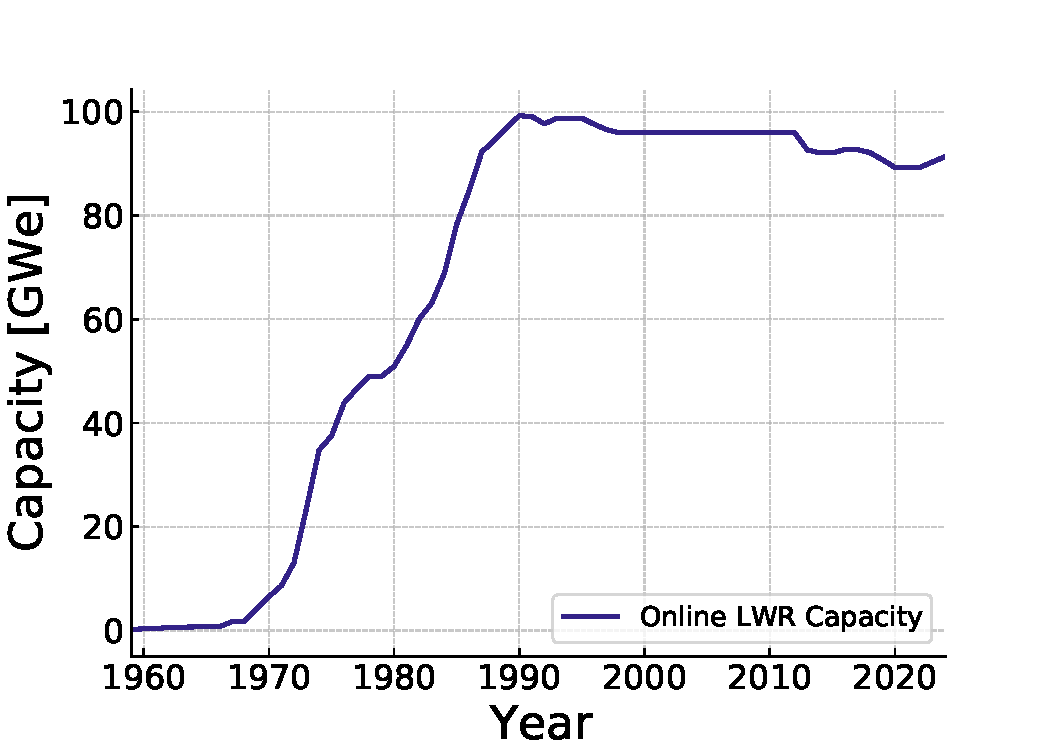
\includegraphics[scale=0.8]{images/intro/online_lwr_cap_2024.pdf}
    \caption{US LWR Capacity through 2024 \cite{IAEA_PRIS}}
    \label{fig:online_lwr_cap_2024}
\end{figure}

According to the \gls{eia}, nuclear energy made up 18\% of utility-scale electricity generation in 2023 \cite{eia_elec_gen_2024}, which makes it 46.5\% of total clean energy generation and the largest producer of clean energy in the country. The last license expiration is now 2063 with the completion of Vogtle Unit 4, but, to meet our growing energy demands and replace the current fleet as it retires over the next several decades. The \gls{us} will need to deploy new reactors at a rate that has not been seen since the 1970s. The \gls{doe} has published a liftoff report on the potential for nuclear energy to meet the demands of the future, and has outlined a variety of scenarios that could lead to a 100\% clean energy future by 2050 \cite{julie_liftoff_pathways_2024}. One of the striking takeaways from the liftoff report is the potential demand for nuclear to triple by 2050 due to new capacity demand, the retirement of fossil fuels, electrification of our economy, and other behind-the-meter applications of nuclear technologies. The potential that \gls{doe} outlines is not without its challenges; the \gls{eia} 2023 Domestic Uranium Production Report highlights the decrease in uranium concentrate production in the \gls{us} and the number of fuel cycle facilities that are dormant or have been decommissioned \cite{eia_uranium_statistics_2023}.

Despite these deployment challenges, the \gls{doe} liftoff report asserts that high-value propositions in low land use, firm energy generation, direct heat applications, local economic benefits, and the low transmission build-out associated with nuclear energy make it a compelling choice. Some of these benefits can be reflected in the 73\% increase in uranium production workers from 2022 to 2023, the 4x increase in exploration of uranium resources, and \$20 million increase in resource investment \cite{eia_uranium_statistics_2023}.

The current fleet of \gls{lwr}s has been the backbone of the commercial nuclear industry, but we are on the precipice of a different generation of reactor technologies. The fleet of \gls{lwr}s uses a ceramic uranium-oxide fuel that is enriched to 3-5\% $^{235}$U, but there is a panoply of advanced reactor designs that are at various stages of deployment making use of our decades of experience with nuclear energy. These reactors vary in size from large gigawatt-scale reactors to smaller reactors that can fit on the back of a truck. The design space for these reactors is vast, but one innovation that has been a focus of the nuclear industry is the \gls{triso} fuel particle. This fuel particle is a small sphere of uranium fuel that is coated in layers of carbon and silicon carbide. \gls{triso} is designed to be more robust than traditional fuel and can be used in a variety of reactor designs that require higher enrichments of $^{235}$U, potentially into \gls{haleu} territory (5-20\%).

The \gls{nfc} describes the plethora of steps nuclear fuel goes through
in its life cycle. In Figure \ref{fig:once-through} we have outlined a
simple "once-through" fuel cycle (so-called because the fuel goes through
the cycle once in its lifetime). The fuel cycle begins with mining uranium ore, typically from uraninite or pitchblende deposits. We then mill and refine the ore into yellowcake, which we convert into uranium hexafluoride. We enrich the uranium hexafluoride to the desired level of $^{235}$U, and then convert it into uranium dioxide. We fabricate the uranium dioxide into fuel pellets, which we load into fuel rods. We then load the fuel rods into the reactor, using them to generate heat. The heat generates steam, which drives a turbine and generates electricity. We then remove the spent fuel from the reactor and store it in a spent fuel pool, where it cools down. After a period of time, we move the spent fuel to dry cask storage, where it will remain until we find a long-term solution.

\begin{figure}[h]
    \centering
    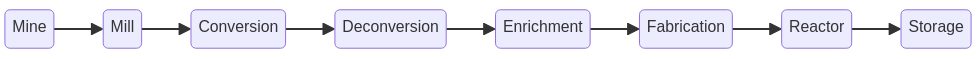
\includegraphics[scale=0.40]{images/once_through_fc.png}
    \caption{US Once-through Fuel Cycle}
    \label{fig:once-through}
\end{figure}

Although we have linearly presented them, these steps are interwoven with international relationships, and long-term purchasing agreements that complicate the establishment of new supply chains. As a consequence, the availability of services at each step in the fuel cycle is difficult to model; this is where we make use of the \cyclus \cite{huff_cyclus_intro_2016} tool. \cyclus is a nuclear fuel cycle simulator that allows users to model the movement of material between facilities in a discrete-event simulation. These facilities are run by agents that make decisions and interact with other agents. Because \cyclus is designed to be technology agnostic, we can use it to model a variety of fuel cycles and reactor types--although it is not primarily a physics code, and coupling it with true physics code can be necessary for some problems.

Partners in industry, academia, and government are building the body of literature surrounding \gls{triso} fuel cycles. This work is a timely evaluation of a variety of energy-demand scenarios and an optimization of the deployment of advanced reactors building off of the method established by Bachmann et \textit{al.} \cite{bachmann_enrichment_2021} for \gls{haleu} fuel, incorporating the staggered enrichment demand that some advanced reactor companies have announced they will explore as the \gls{haleu} supply chain develops. We seek to understand the deployment of advanced reactors in the \gls{us} and the implications of the fuel cycle on the deployment of these reactors as some designs adopt a staggered enrichment demand. We have chosen to focus on a few key metrics to understand the performance of each deployment scenario. These metrics are: \gls{swu}, energy output, mass of fuel, isotopic composition, and reactor deployment. In service of this goal, we will also examine the computational efficiency of the \gls{dre} in \cyclus to contribute to a robust tool for future analysis.


\pagebreak

(in progress, will update as the thesis comes together)
The structure of this thesis is as follows:

\begin{itemize}
    \item Chapter 2
\end{itemize}